\begin{enumerate}
	\item Wzory Cramera przy rozwiązywaniu równań liniowych;
	\item liczenie objętości \(n\)-wymiarowego równoległościanu (opisanego wektorami znajdującymi się w kolejnych wierszach macierzy)
	\item jeśli wyznacznik macierzy jest niezerowy to wiemy, że ma ona odwrotność.
\end{enumerate}

\begin{figure}[h]
	\centering
	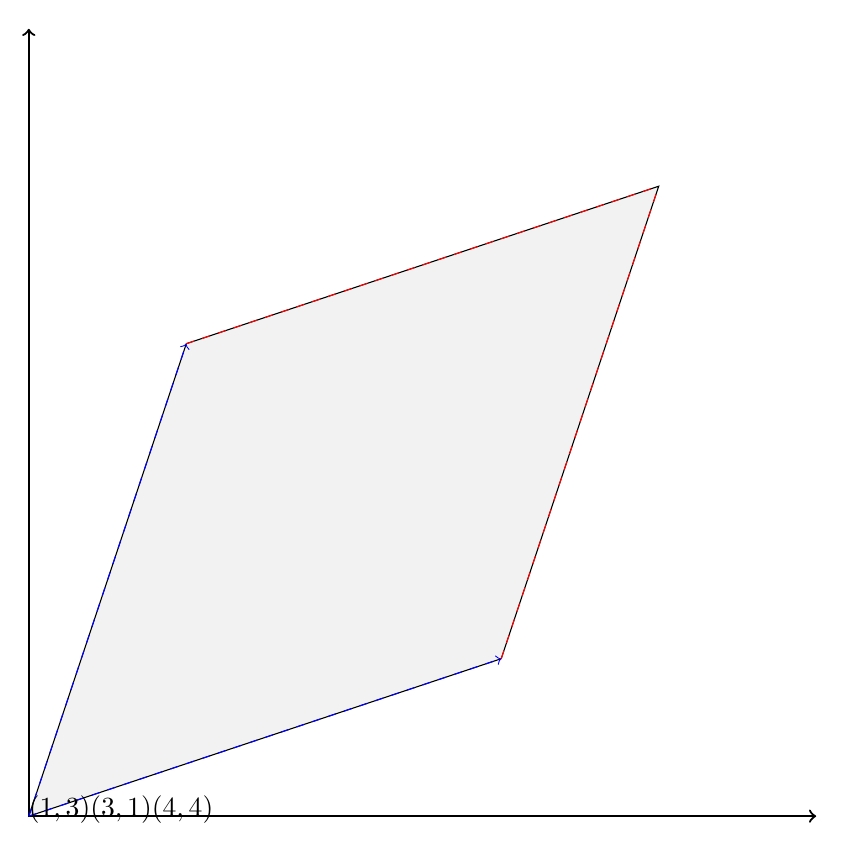
\begin{tikzpicture}[scale=2]

		\filldraw[fill=black,fill opacity=0.05] (0,0) -- (3,1) -- (4,4) -- (1,3) -- (0,0) -- cycle;

		\draw[thick, ->] (0,0) -- (5,0);
		\draw[thick, ->] (0,0) -- (0,5);

		\draw[dashed, blue, ->] (0, 0) -- (3, 1);
		\draw[dashed, blue, ->] (0, 0) -- (1, 3);

		\draw[dashed, red, -] (3, 1) -- (4, 4);
		\draw[dashed, red, -] (1, 3) -- (4, 4);

		\tkzDefPoint(1,3){A};
		\tkzLabelPoint[above, black](A){\((1, 3)\)};

		\tkzDefPoint(3, 1){B};
		\tkzLabelPoint[below, black](B){\((3, 1)\)};

		\tkzDefPoint(4, 4){C};
		\tkzLabelPoint[above, black](C){\((4, 4)\)};

	\end{tikzpicture}
	\caption{Dwuwymiarowa figura geometryczna wyznaczona parą wektorów \((1, 3)\) i \((3, 1)\). Jeśli obliczymy wartość \( \det{\begin{bmatrix}  1 & 3 \\ 3 & 1 \end{bmatrix}} \) to wyjdzie nam \(-8\) (a więc po wzięciu wartości bezwzględnej dostaniemy \(8\), i to jest w istocie pole tej figury). Ale śmieszne!}
\end{figure}